\section{Experiments}
\label{sec:experiments}

\subsection{Data and Experimental Scope}
We analyze 438 our TRELLIS-generated reconstructions associated with 50 IMPACT
patents~\cite{shomee2024impact}. The corresponding archive contains 3,504 rendered
view records and 433 generation logs. These counts describe the local archive,
not the entire IMPACT dataset. The original selection procedure and a geometric
ground-truth mesh set are unavailable. We do not interpret this convenience
sample as a representative estimate of all patent categories.

The new adaptation implementation supports reviewed figure crops and patent-disjoint
development and test manifests; a completed held-out evaluation is not available. Its code rejects a patent occurring in both
splits within one manifest. Crop rules and preprocessing parameters must be
fixed on development patents before test scoring. The currently prepared pilot
contains one reviewed drawing from D0908314; its GPU ablation results have not
been supplied. Historical whole-TIFF results are not substituted for a matched
cropped-input baseline.

\subsection{Implementation Details}
\label{sec:implementation}
The generator is \texttt{microsoft/TRELLIS-image-large}; the original generation scripts use
seed 1 and default sampling parameters. The new experiment pairs seeds across
four branches and supports repeated seeds. Prepared crops use a white
$518\times518$ canvas. Provisional development settings are distance support
$\sigma_d=2$ pixels and smoothing $\sigma_g=1$ pixel. These are implementation
settings, not empirically selected optimum values. All branches use the same
checkpoint and mesh export arguments: \texttt{simplify=0.95} and a 1024-pixel
texture. The exact checkpoint revision, attention backend, and hardware must be
reported with completed runs.

Evaluation uses eight horizontal azimuths spaced by $45^{\circ}$, elevation
$10^{\circ}$, camera radius 3.2, and vertical field of view $40^{\circ}$. Geometry
is centered and scaled to longest extent two. Rendering defaults to
$512\times512$ pixels with a white background and fixed illumination.
Reference and render images undergo the evaluator's independent crop-and-center
procedure. This removes framing differences but does not register pose.

\paragraph{Metrics and uncertainty.}
We report RGB SSIM~\cite{wang2004ssim}, PSNR, AlexNet-based
LPIPS~\cite{zhang2018lpips}, and normalized image/image and caption/image CLIP
similarity~\cite{radford2021clip}. CLIP defaults to ViT-B/32; captions are used
only for evaluation. Main summaries average views within each output and weight
patents equally. Completed matched runs additionally average seeds within each
drawing and use 2,000 paired patent-bootstrap resamples for difference intervals.
We omit silhouette IoU and contour distance from performance claims until their
masks are validated. No metric here is a direct ground-truth 3D error.

\subsection{Measured Archive Results}
Table~\ref{tab:archive_results} reports the verified image-based measurements
for the completed TRELLIS generation set. Values average the eight view scores within
each drawing, then drawings within each patent. The final mean and sample
standard deviation give equal weight to each of the 50 patents.

\begin{table}[t]
\centering\small
\caption{Measured evaluation of our TRELLIS-generated outputs: 438 drawings from
50 patents. Values are mean $\pm$ sample standard deviation across patents.
These single-pipeline archive measurements are not a matched comparison of
adaptation configurations.}
\label{tab:archive_results}
\begin{tabular*}{\columnwidth}{@{\extracolsep{\fill}}lr@{}}
\toprule
Metric & Mean $\pm$ SD \\
\midrule
SSIM $\uparrow$ & $0.6506\pm0.1392$ \\
PSNR (dB) $\uparrow$ & $11.9105\pm2.6989$ \\
LPIPS $\downarrow$ & $0.5316\pm0.1286$ \\
CLIP image similarity $\uparrow$ & $0.7130\pm0.0381$ \\
CLIP caption similarity $\uparrow$ & $0.2408\pm0.0197$ \\
\bottomrule
\end{tabular*}
\end{table}

The metrics characterize agreement between line drawings and shaded renders,
not direct geometric error. Their variation reflects differences in drawing
style, content, framing, and pose as well as generated appearance. These
historical whole-TIFF results cannot serve as the stock row of a new experiment
using reviewed crops and matched seeds. No independently measured SketchDream
or Know3D comparison is available for these inputs, and no superiority over
those methods is claimed.

\subsection{Adaptation Configurations}
\label{sec:ablations}
Table~\ref{tab:components} describes the implemented configurations without introducing
additional model weights. The stock/bypass comparison tests the effect of the
backbone preprocessing on identical RGB inputs. Bypass/distance tests the
structural map, and distance/smoothing tests the additional smoothing step.
Keeping this sequence explicit prevents benefits from reviewed crops or backend
changes from being attributed to a different component.

\begin{table}[t]
\centering\small
\caption{Configuration design, not measured ablation results. Entries identify enabled operations;
matched reconstruction evaluation is not yet complete. All rows share the same reviewed crops, model, export
settings, and paired seeds.}
\label{tab:components}
\begin{tabular*}{\columnwidth}{@{\extracolsep{\fill}}lccc@{}}
\toprule
Branch & Removal & Map & Blur \\
\midrule
Stock & Yes & No & No \\
Bypass & No & No & No \\
Distance & No & Yes & No \\
Distance + blur & No & Yes & Yes \\
\bottomrule
\end{tabular*}
\end{table}

\begin{figure}[t]
\centering
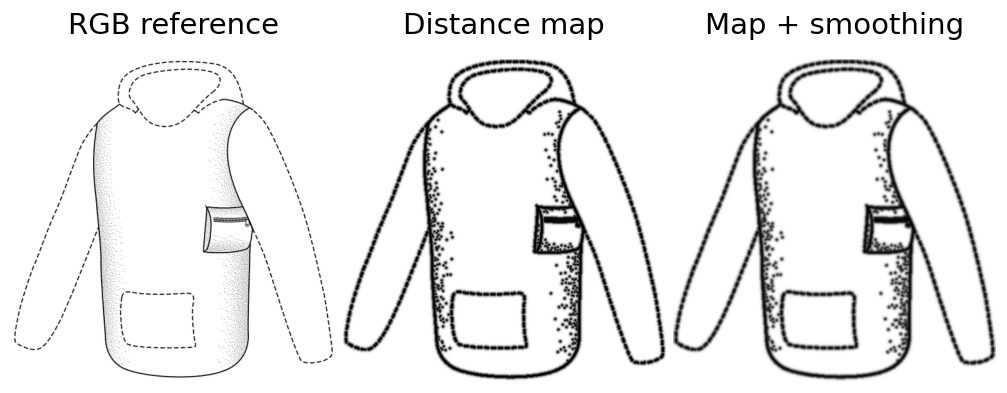
\includegraphics[width=\columnwidth]{figures/input_ablation.png}
\caption{Actual prepared inputs for D0908314: the common RGB reference, the
distance-to-ink representation, and its smoothed variant. The maps preserve and
expand line support, including stippled shading. This is an input-representation
ablation, not evidence of improved reconstruction.}
\label{fig:input_ablation}
\end{figure}

\subsection{View-Coverage Diagnostic}
Unlike the pending adaptation runs, view-subset analysis can be computed directly
from the recorded archive. We compare azimuth $0^{\circ}$ alone, the opposed pair
$\{0^{\circ},180^{\circ}\}$, four orthogonal views, and all eight views. The same
438 drawing/model pairs are retained. Table~\ref{tab:view_subsets} contrasts mean
scores with best-view SSIM; Figure~\ref{fig:view_sensitivity} shows per-azimuth
variation. A larger best-view score can arise from searching more views and does
not establish a better generated mesh. This diagnostic varies evaluation
coverage, not the number of conditioning views or a view-aware generation module.

\begin{table}[t]
\centering\small
\caption{View-subset diagnostic on our generated reconstruction set (438 drawings, 50 patents). Subsets are fixed before scoring. Values are patent-level means; best SSIM selects a view separately for each drawing. This changes evaluation coverage, not generation.}
\label{tab:view_subsets}
\begin{tabular*}{\columnwidth}{@{\extracolsep{\fill}}lrrr@{}}
\toprule
Views & Mean SSIM & Best SSIM & LPIPS \\
\midrule
1 & 0.6356 & 0.6356 & 0.5422 \\
2 & 0.6389 & 0.6496 & 0.5411 \\
4 & 0.6586 & 0.6998 & 0.5287 \\
8 & 0.6506 & 0.7026 & 0.5316 \\
\bottomrule
\end{tabular*}
\end{table}


\begin{figure}[t]
\centering
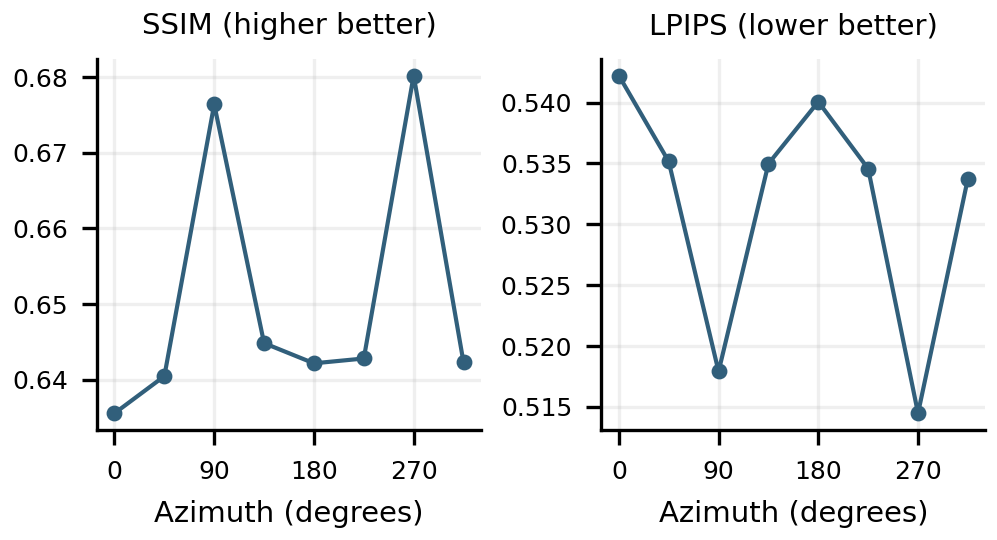
\includegraphics[width=\columnwidth]{figures/view_sensitivity.png}
\caption{Measured view sensitivity in the completed generation set. Each point averages
scores within patents and then across 50 patents. The curves show changes with
render azimuth for the same assets, not adaptation gains or estimated reference
camera poses.}
\label{fig:view_sensitivity}
\end{figure}

\subsection{Mesh and Qualitative Assessment}
Recomputing topology from all 438 GLBs succeeds without parsing errors. Median
vertex and triangle counts are 8,092.5 and 11,580; the median index-connected
component count is 204.5 and median boundary-edge count is 3,800. None passes the
closed-edge incidence test. These values describe the stored representation:
coincident positions are not welded, so seams can inflate connectivity and
boundary counts. They are not directly comparable to processed-mesh counts
without stating the definition.

The manuscript's three existing qualitative examples show patent drawings beside
renders of our TRELLIS-generated assets (Figure~\ref{fig:trellis_comparison}). They are illustrative,
not a random sample or a controlled method comparison. A matched five-drawing
inspection from D0908314 additionally reproduces selected-view SSIM to numerical
precision. Some references contain several figures and labels, and thresholding
saved resized references can remove thin linework. Raw-TIFF validation and
qualitative coverage of additional patents are still required.

\begin{figure}[t]
\centering
\setlength{\tabcolsep}{1pt}
\begin{tabular}{@{}ccc@{}}
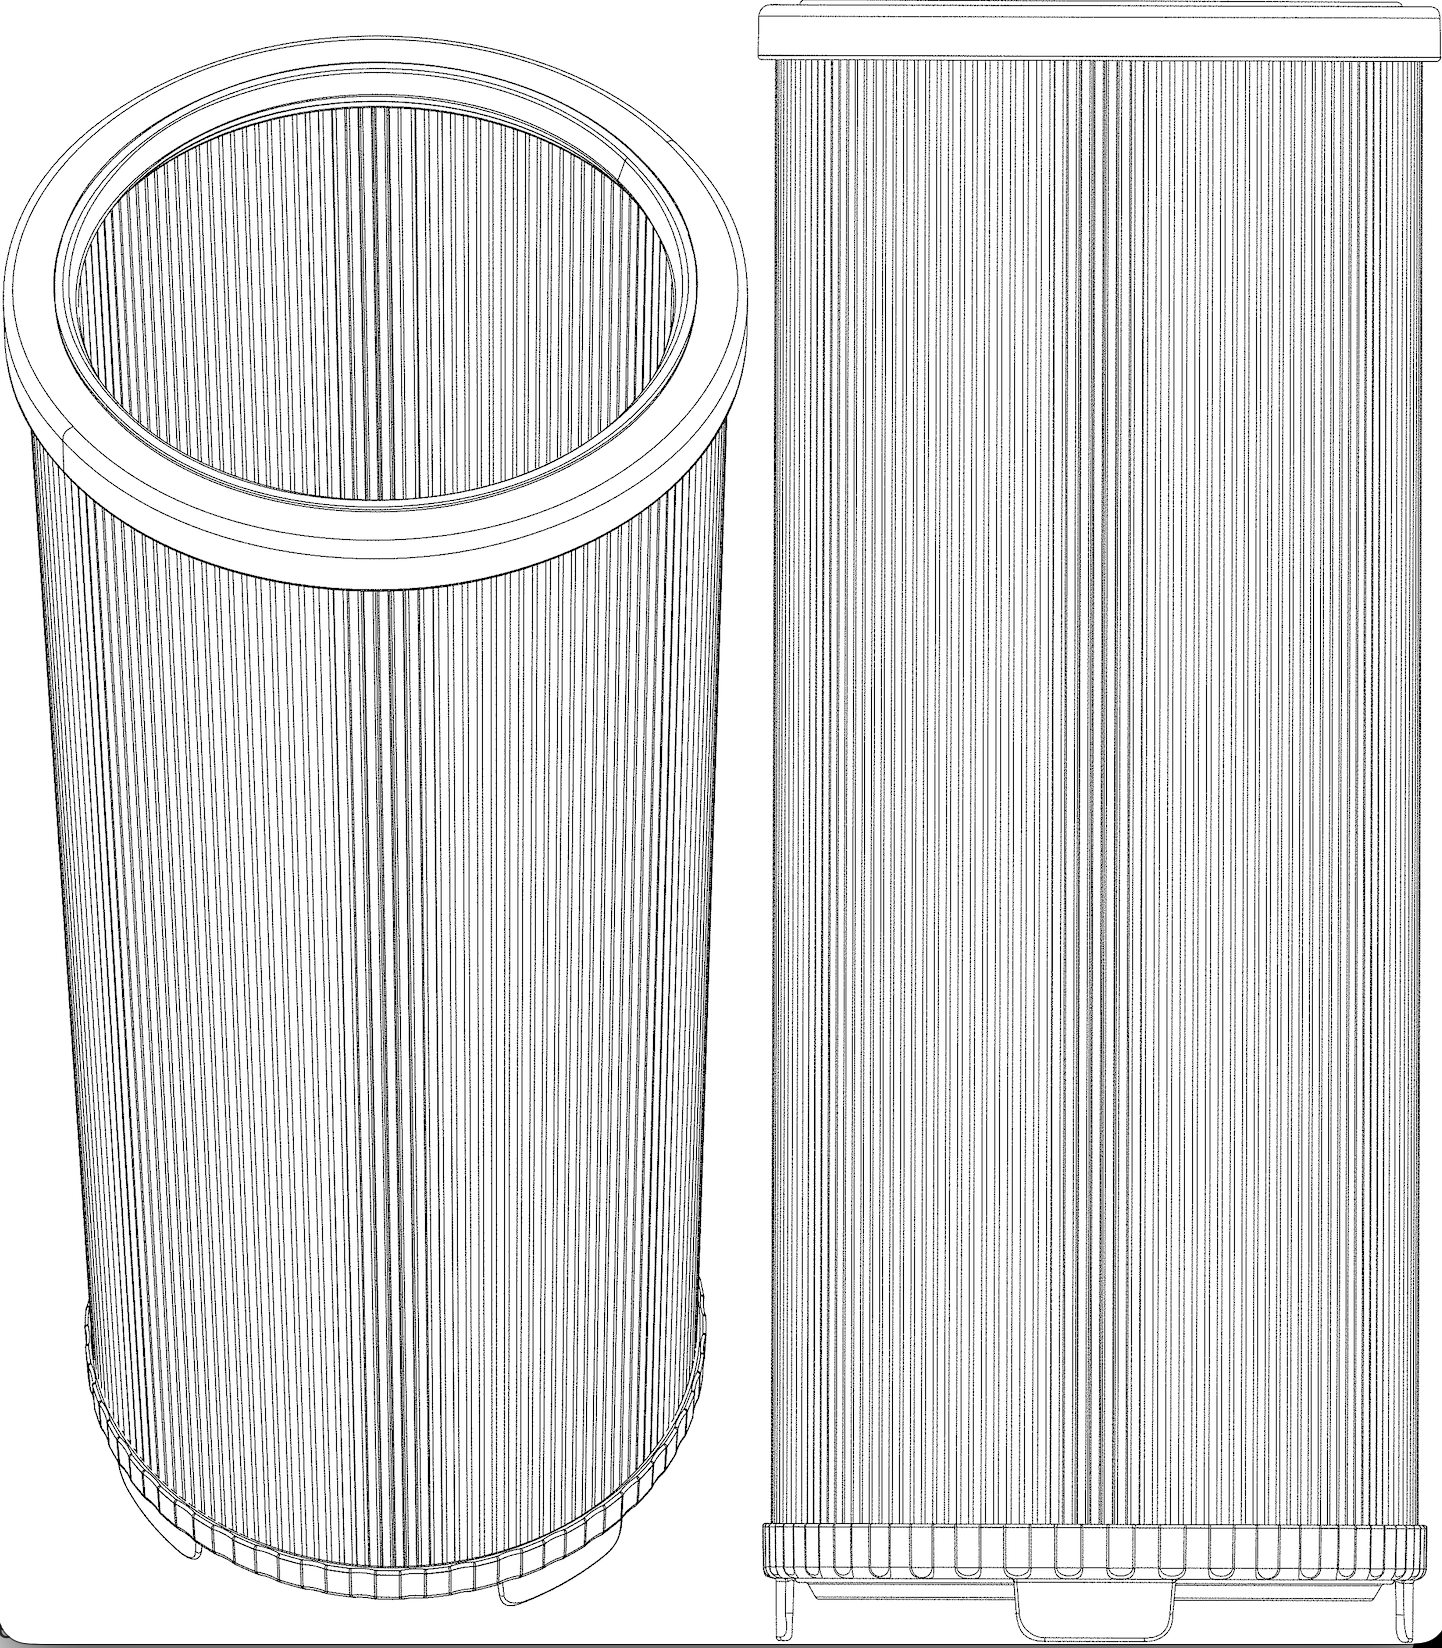
\includegraphics[width=.315\columnwidth,height=2.1cm,keepaspectratio]{Trellis_Results/D0921835_D00000_TIFF.png}&
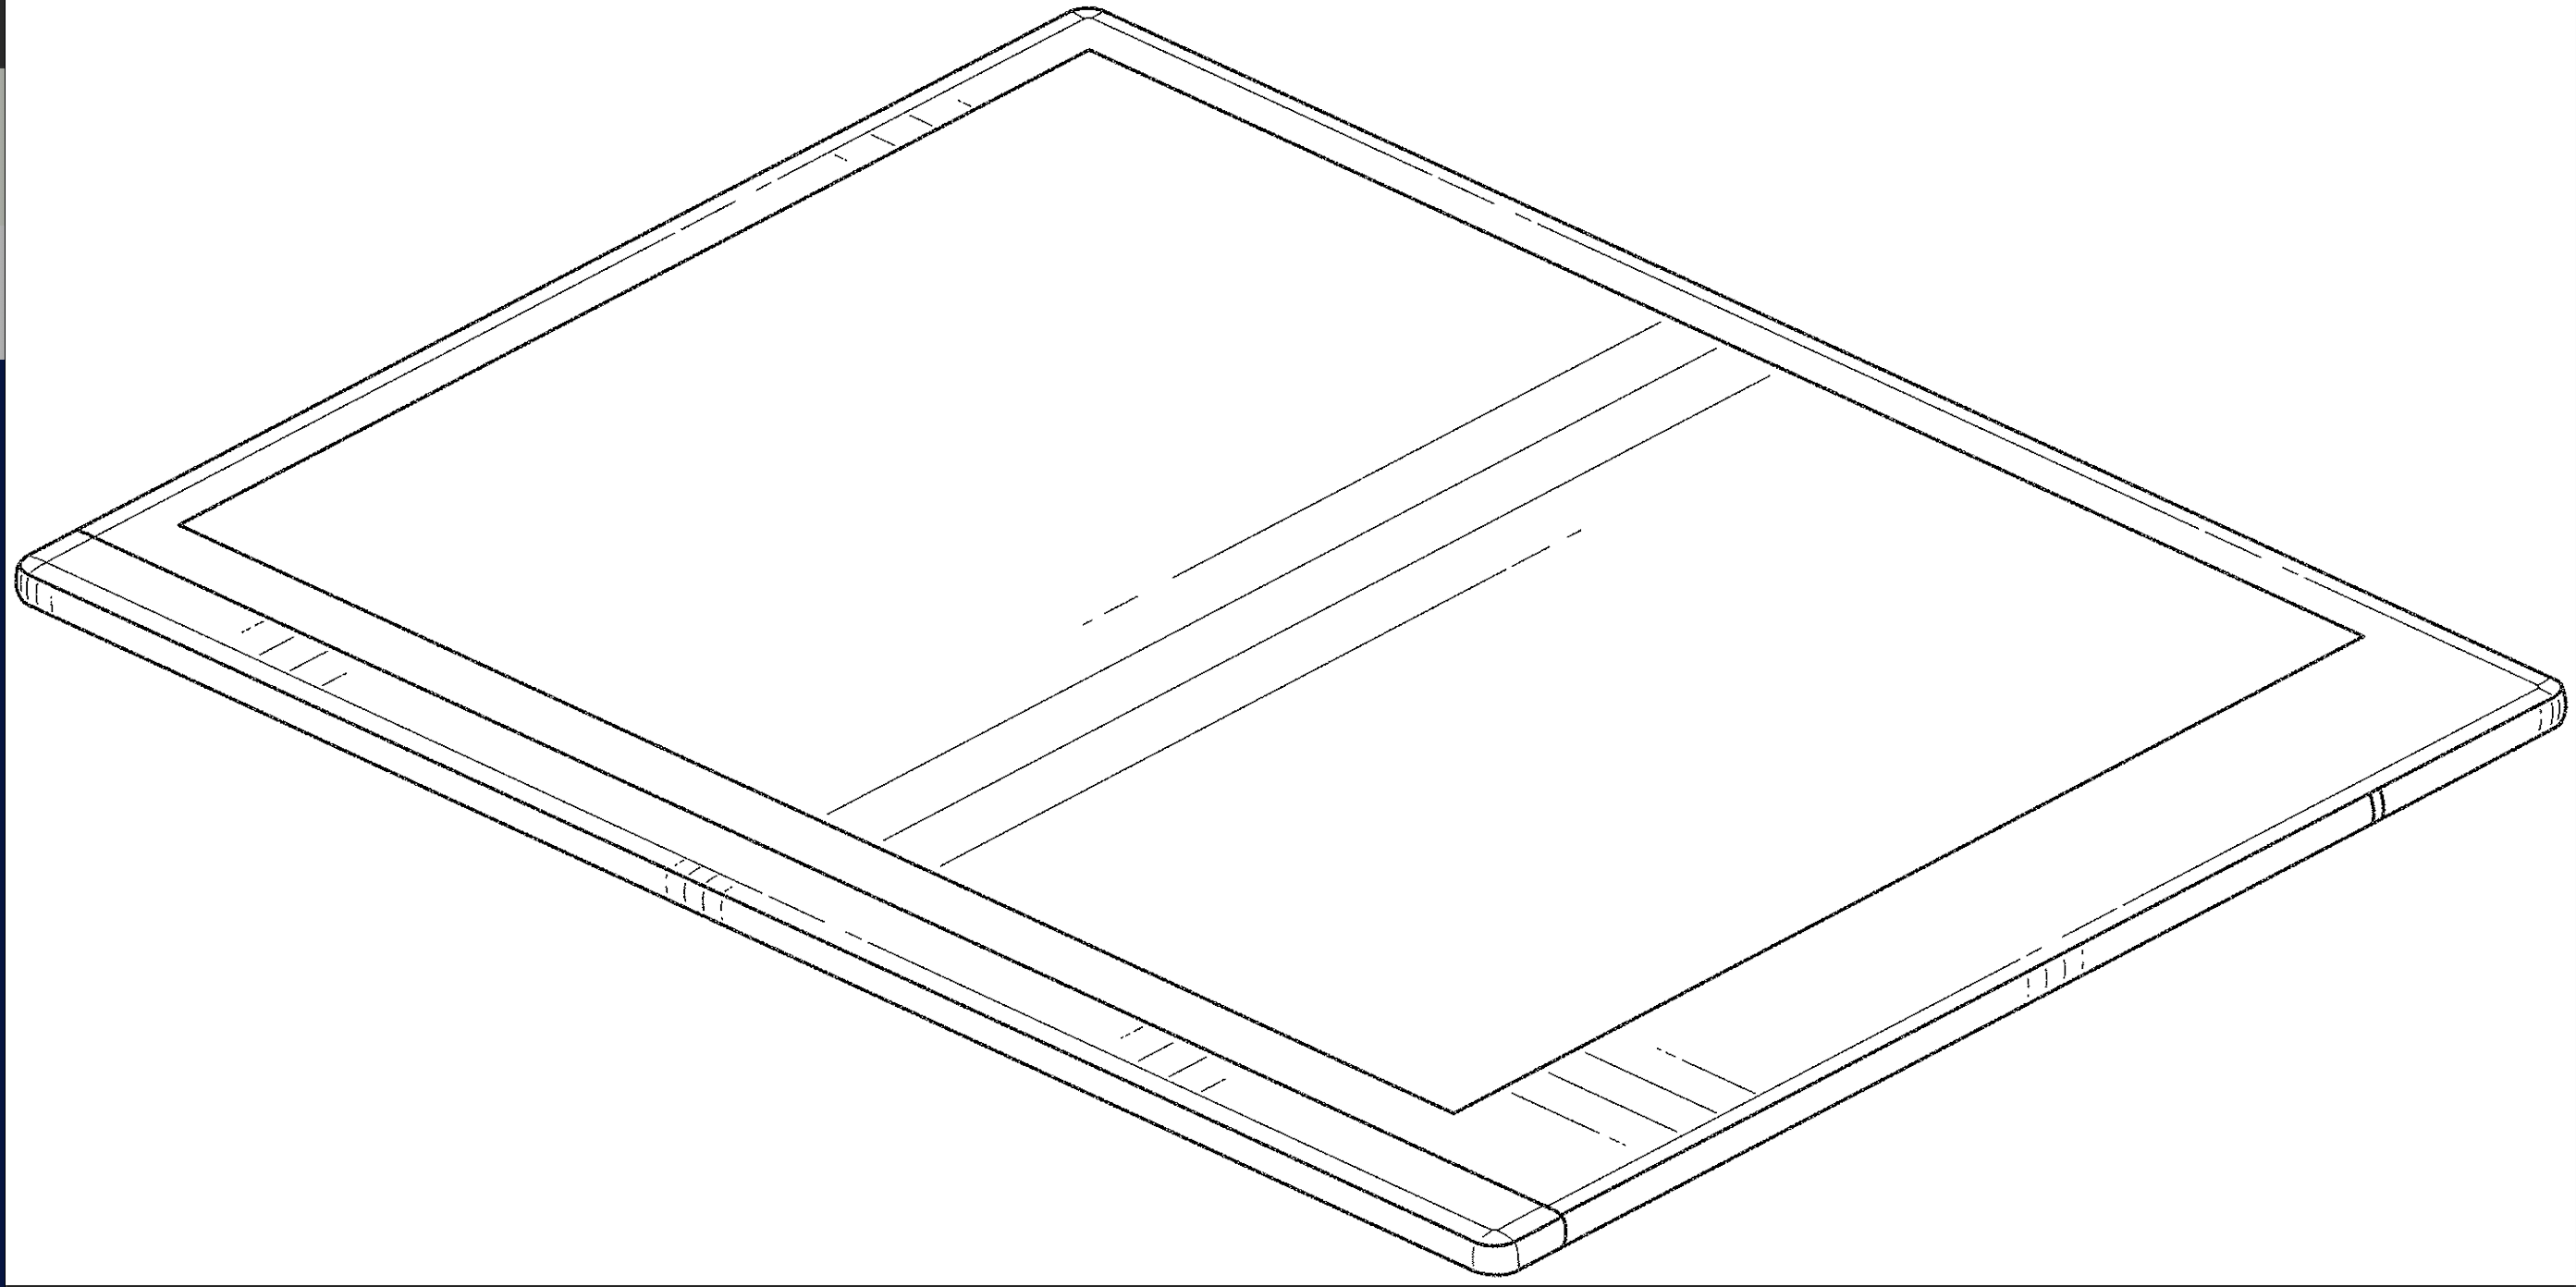
\includegraphics[width=.315\columnwidth,height=2.1cm,keepaspectratio]{Trellis_Results/D0928145_D00000_TIFF.png}&
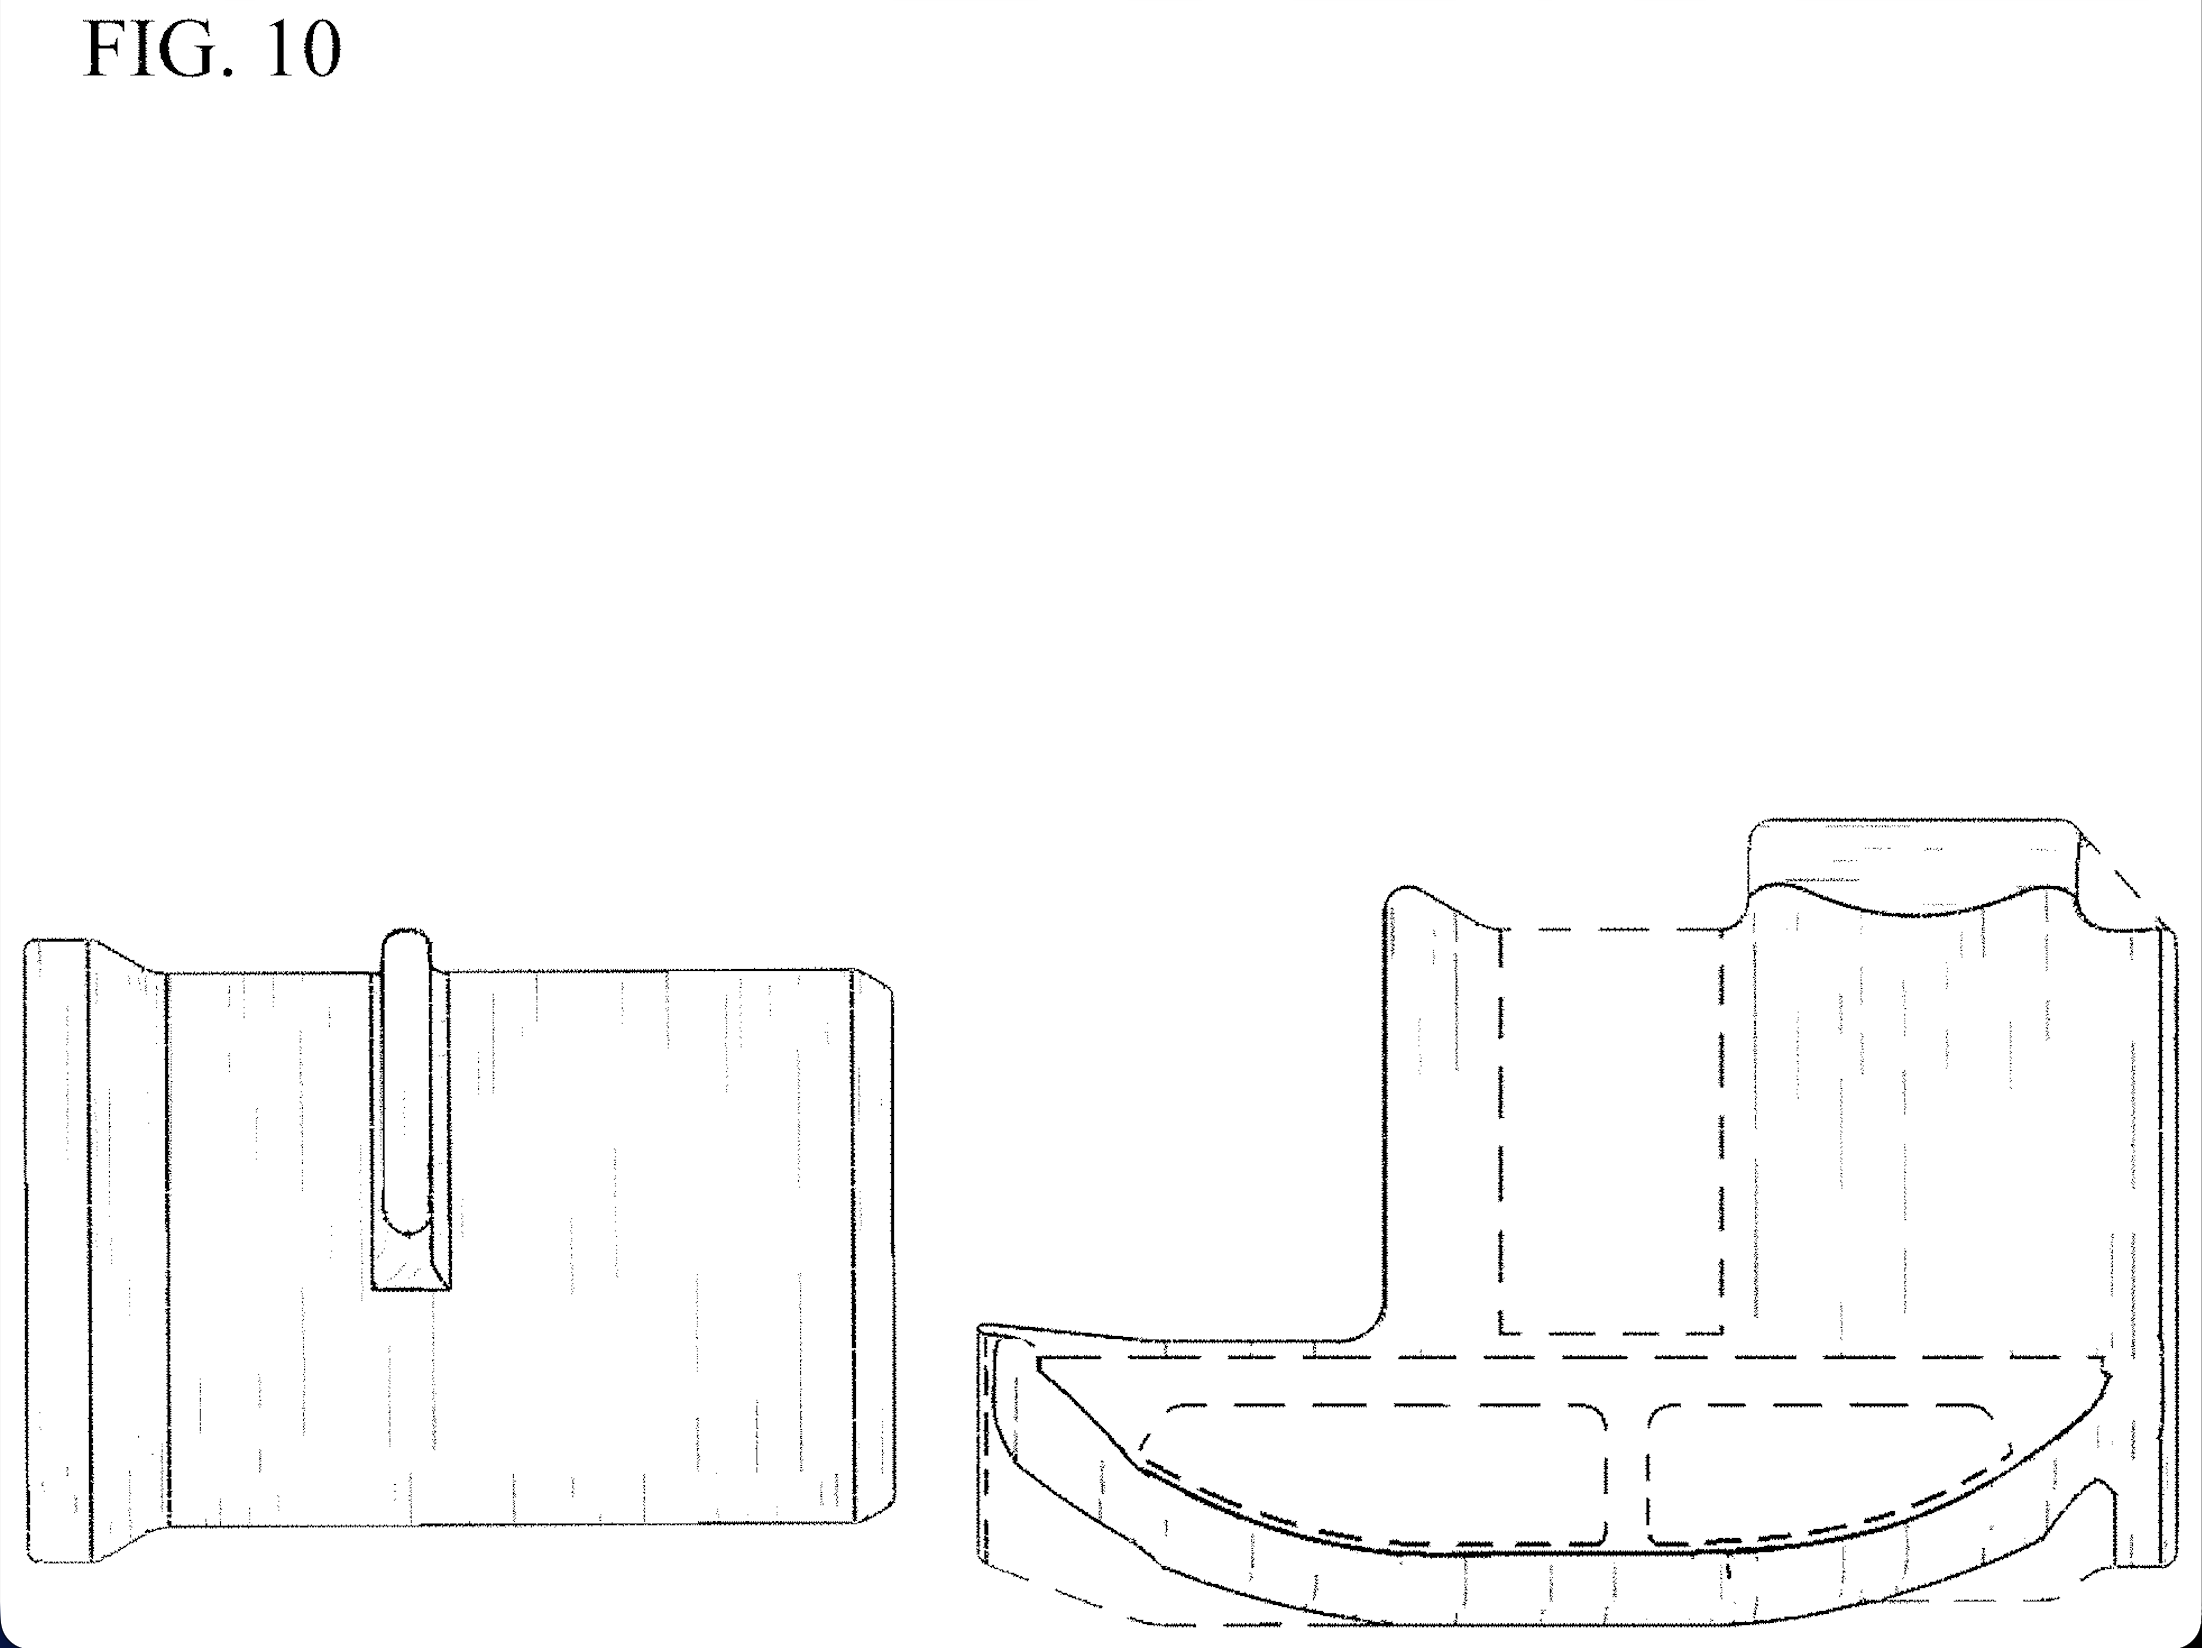
\includegraphics[width=.315\columnwidth,height=2.1cm,keepaspectratio]{Trellis_Results/D0927653_D00010_TIFF.png}\\[3pt]
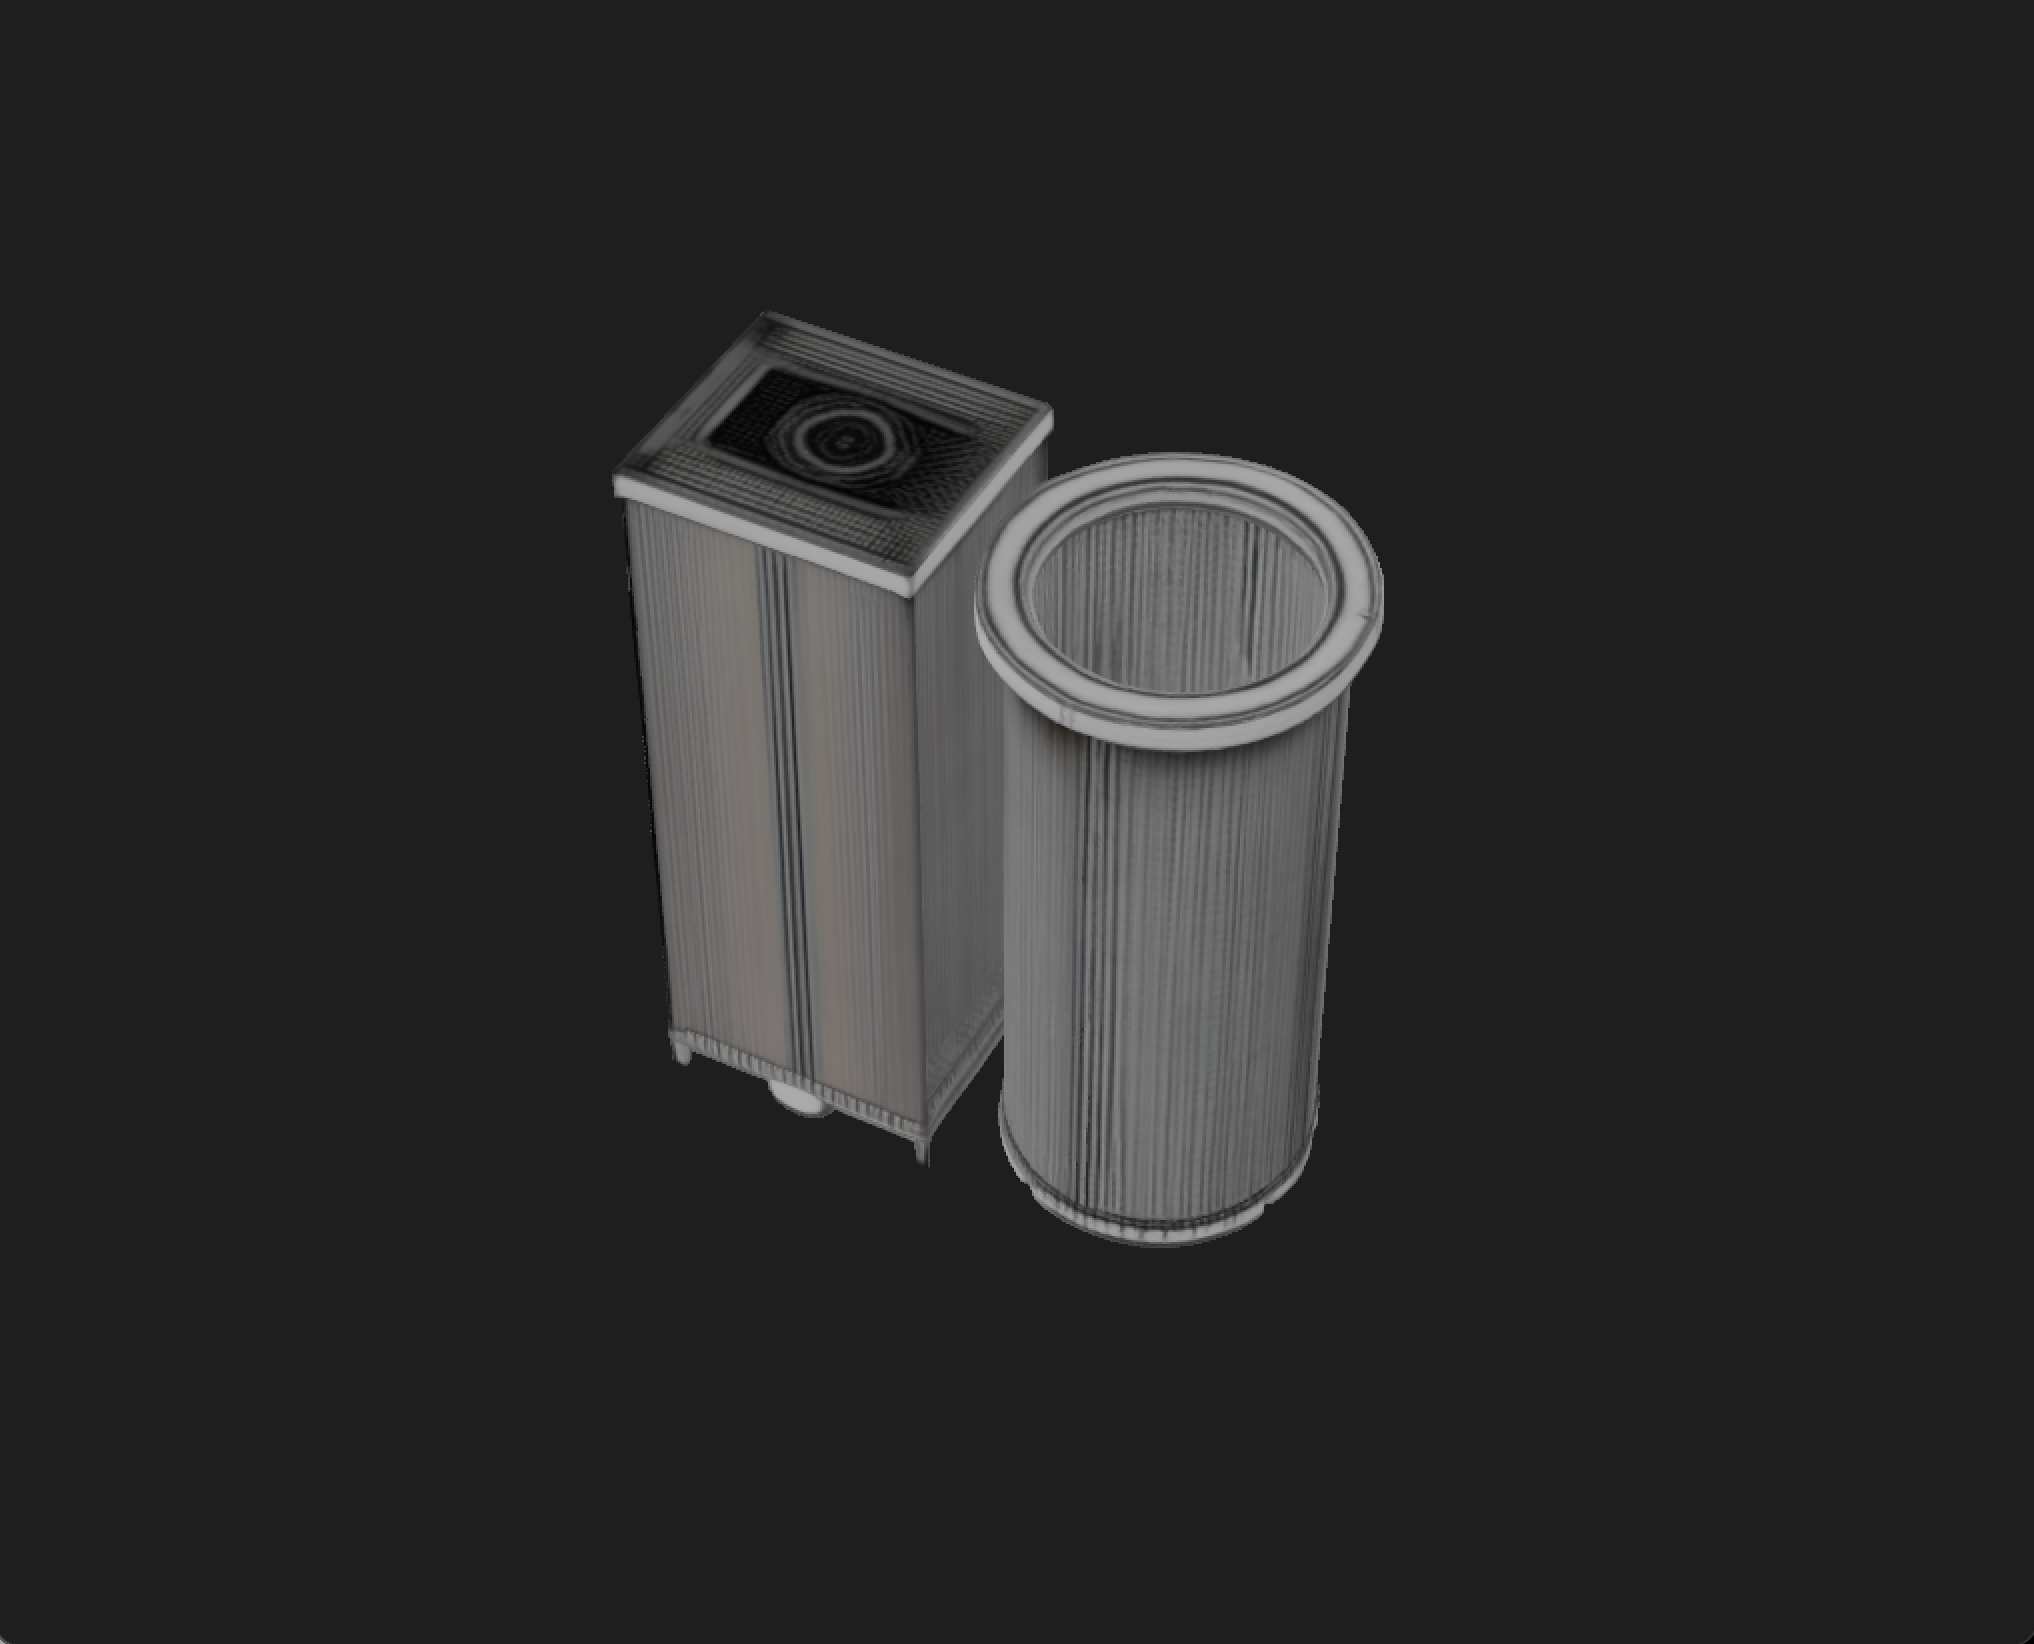
\includegraphics[width=.315\columnwidth,height=2.1cm,keepaspectratio]{Trellis_Results/D0921835_D00000_3D.png}&
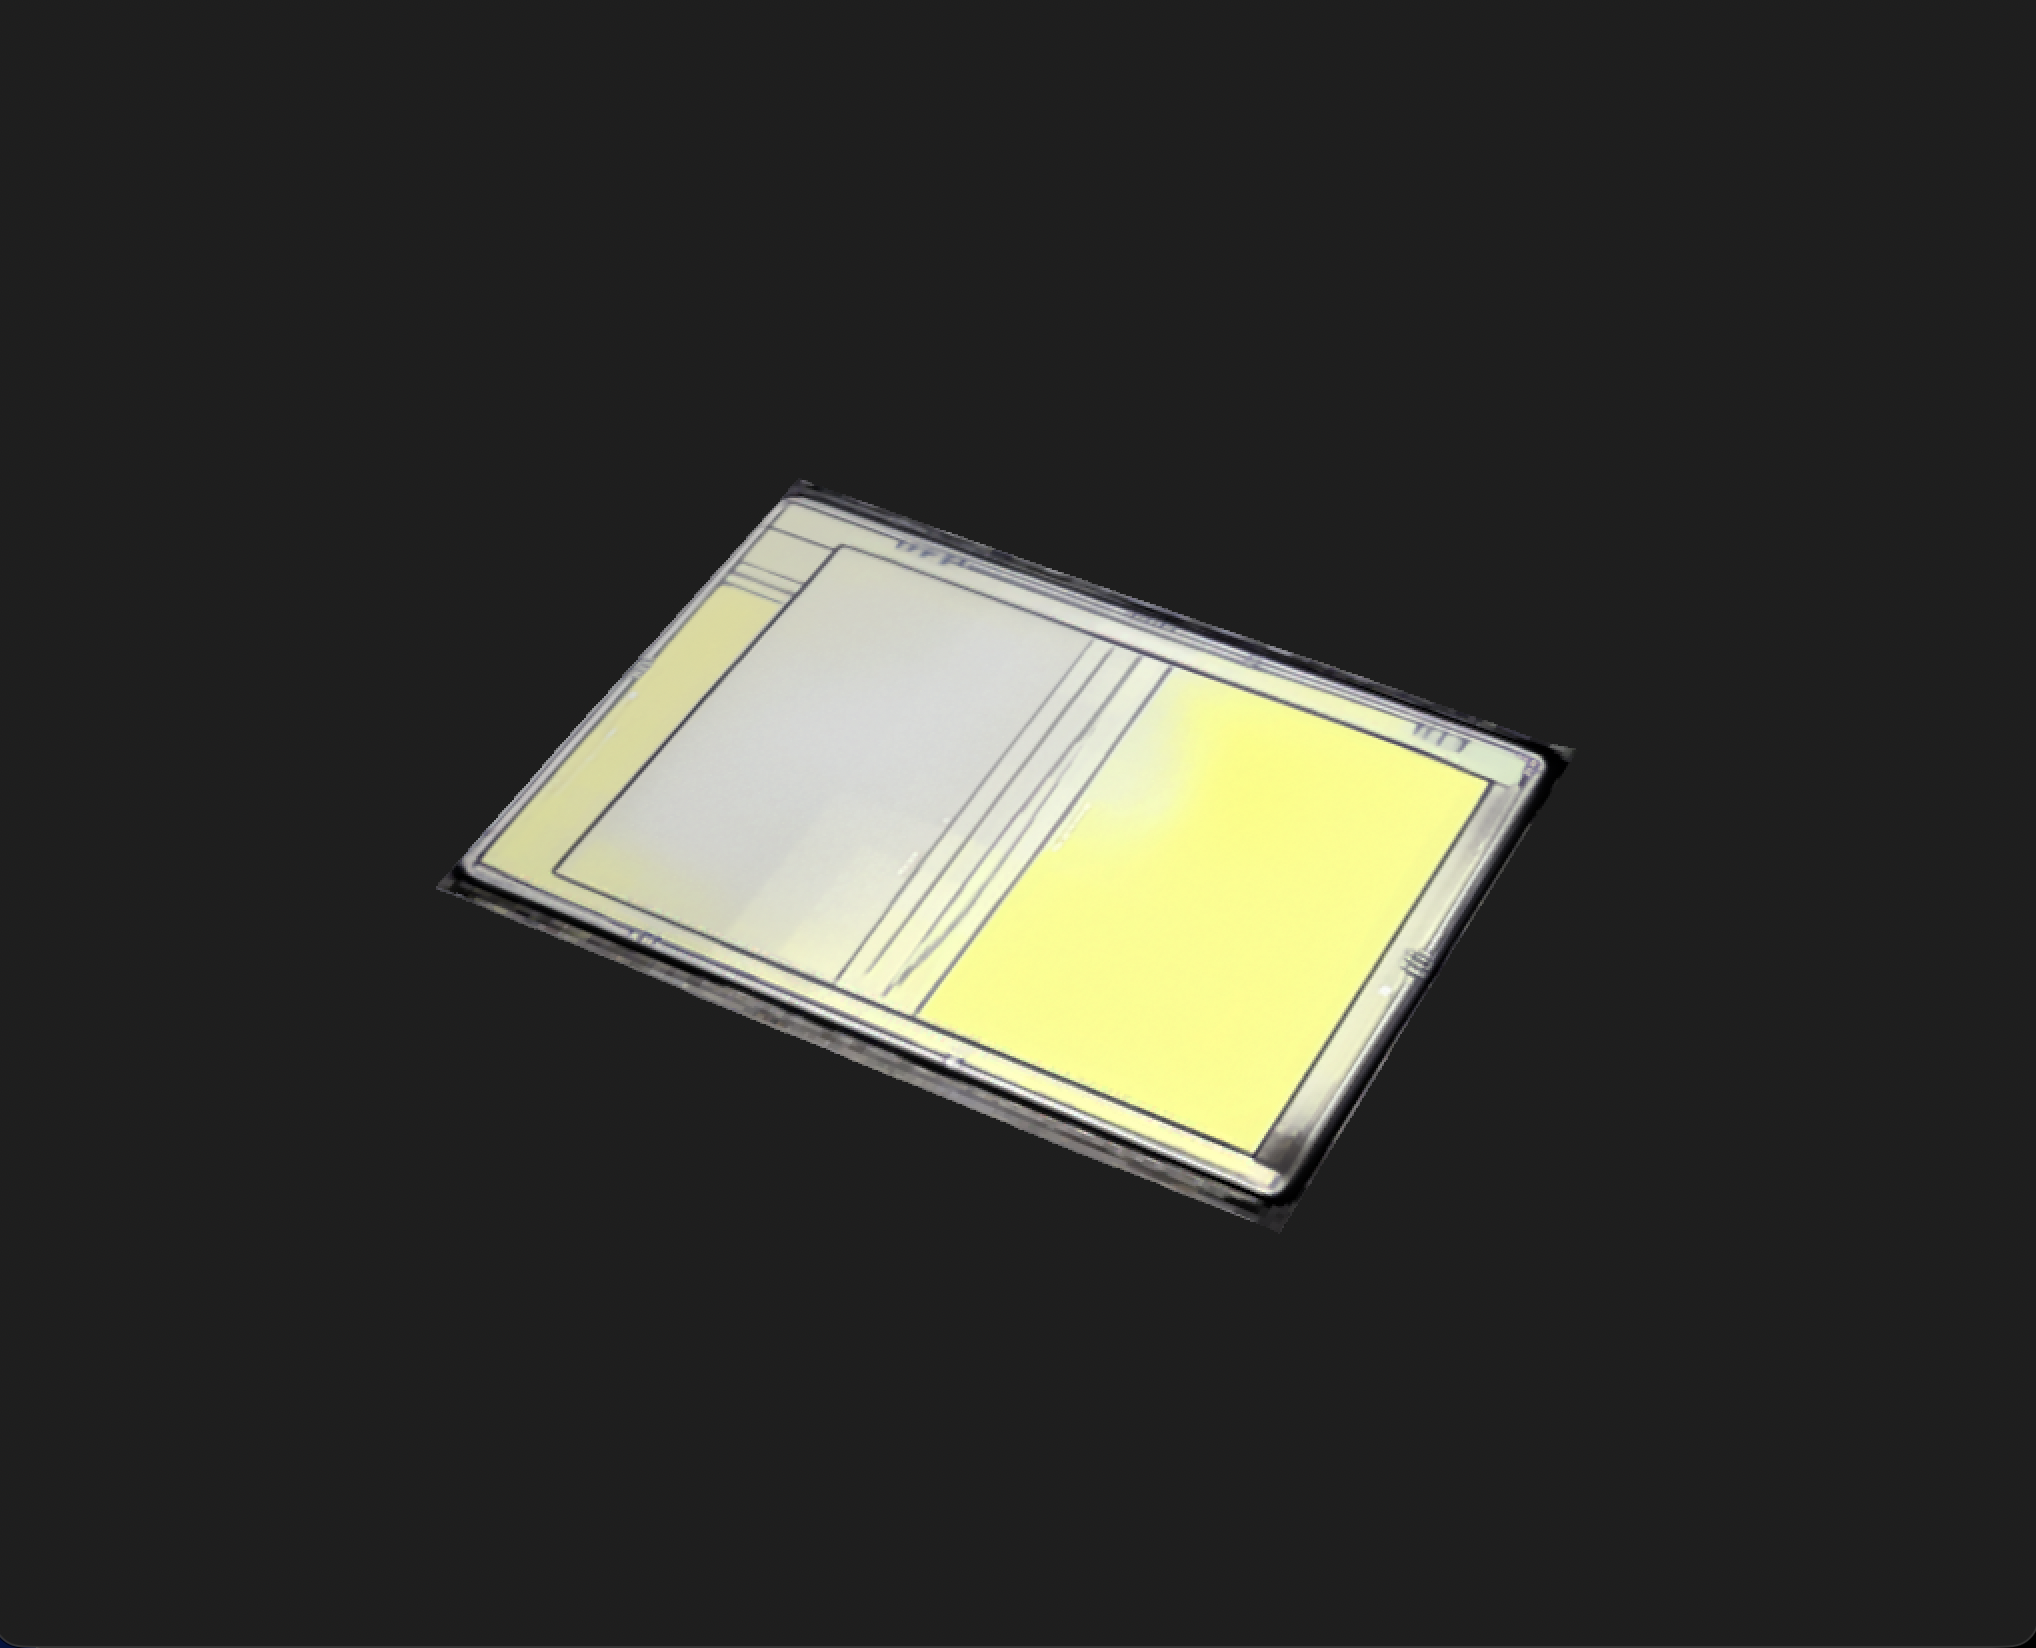
\includegraphics[width=.315\columnwidth,height=2.1cm,keepaspectratio]{Trellis_Results/D0928145_D00000_3D.png}&
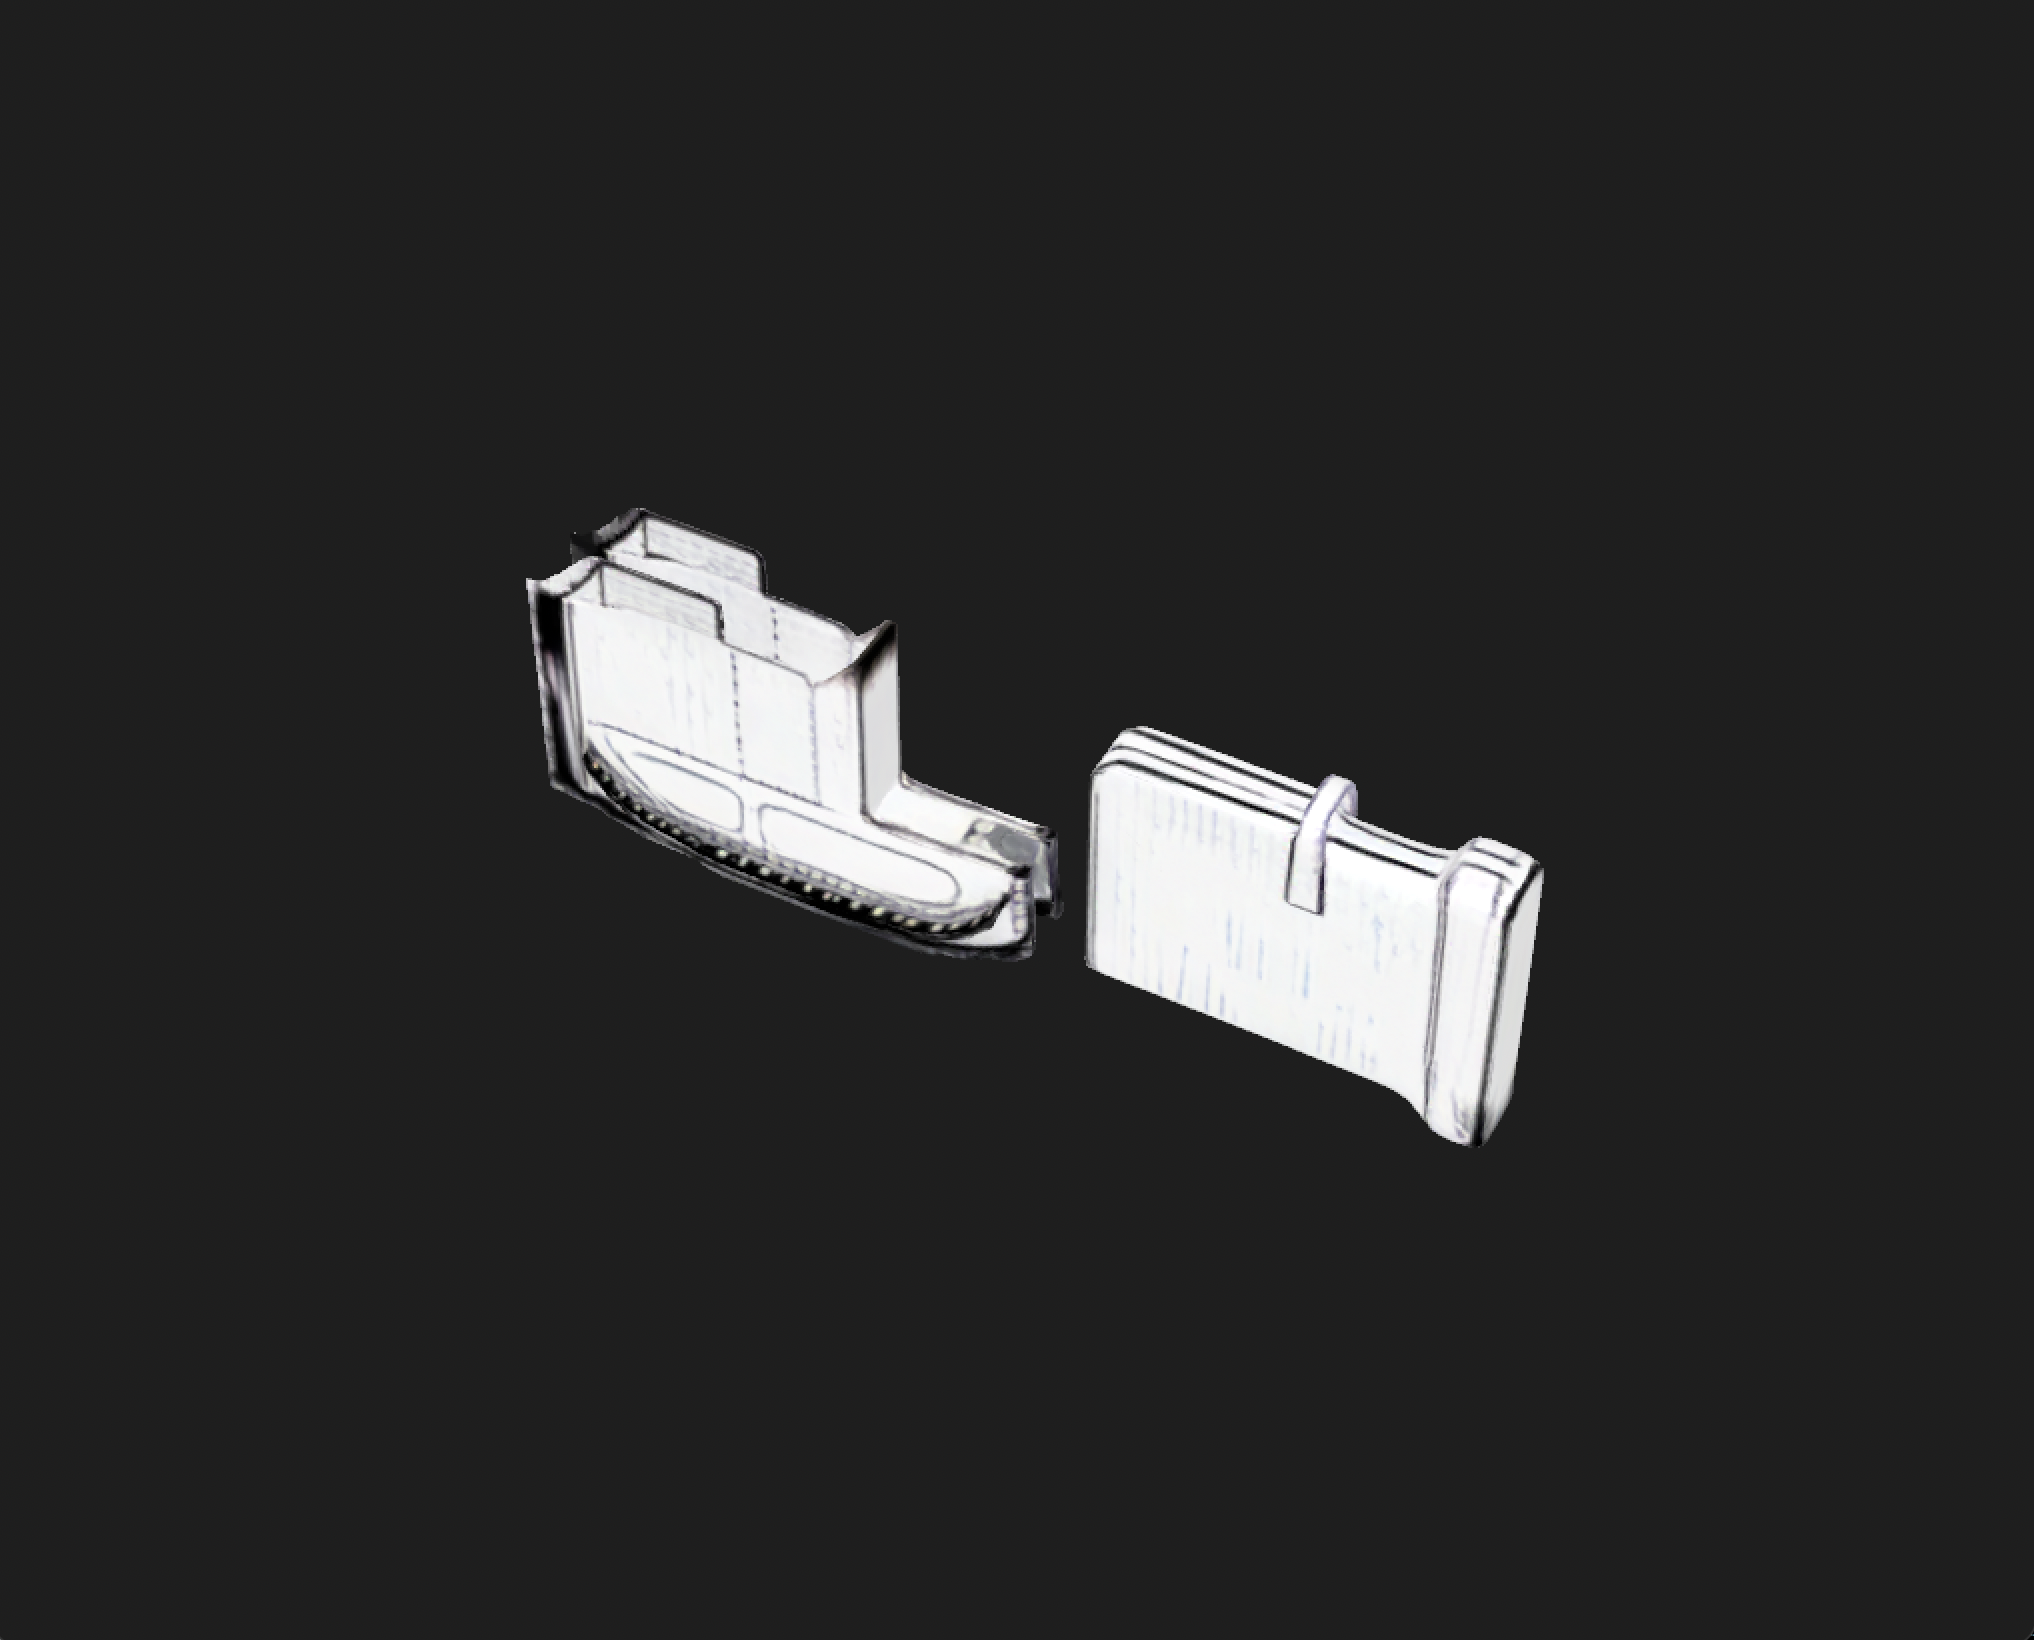
\includegraphics[width=.315\columnwidth,height=2.1cm,keepaspectratio]{Trellis_Results/D0927653_D00010_3D.png}
\end{tabular}
\caption{Existing illustrative patent drawings (top) and renders of our TRELLIS-generated assets
(bottom). These are not outputs of the new adaptation and do not establish a
comparative ranking. The selection is illustrative rather than random.}
\label{fig:trellis_comparison}
\end{figure}
